\documentclass[10pt,letterpaper,notitlepage]{article}
\usepackage[utf8]{inputenc}
\usepackage{amsmath}
\usepackage{amsfonts}
\usepackage{amssymb}
\usepackage{graphicx}
\usepackage{cancel}
\usepackage{float}
\usepackage{hyperref}
\hypersetup{
    colorlinks=true,
    linkcolor=blue,
    filecolor=magenta,      
    urlcolor=cyan,
}
\urlstyle{same}

\usepackage[left=0.75in, right=0.75in, bottom=1.0in,top=0.75in]{geometry}

\numberwithin{equation}{section}

%============================= Put document title here
\newcommand{\DOCTITLE}{Relating Monte Carlo particle tracking to Finite Element Degrees of Freedom
}  

%============================= Macros for equations
\newcommand{\beq}{\begin{equation*}
\begin{aligned}}
\newcommand{\eeq}{\end{aligned}
\end{equation*}}

\newcommand{\beqn}{\begin{equation}
	\begin{aligned}}
\newcommand{\eeqn}{\end{aligned}
	\end{equation}}  


\begin{document}
\noindent
{\LARGE\textbf{\DOCTITLE}}
\newline
\newline
\newline
\noindent
{\Large Your name${^1}$, Someone ElsesName$^{1,2}$}
\newline
\noindent\rule{\textwidth}{1pt}
{\small $^1$ Your affiliation.}
\newline\noindent
{\small $^2$Other affiliation.}
\newline
\newline
\textbf{Abstract:}\newline\noindent
The abstract
\newline
\newline\noindent
{\small
\textbf{Keywords:} error estimation; uncertainty quantification; residual monte carlo}

\section{Introduction}
\subsection{Tracklength as a measure of flux}
The classical definition of flux is that of the number of particles crossing a unit area, however, the alternate definition is the tracklength per unit volume. Using the latter we can apply Monte Carlo tracking to estimate the average tracklength, $\bar{\ell}$, of $N$ amount of particles traveling through (or in) a  computational cell as
\beqn
\bar{\ell} = \frac{1}{N} \sum_{n=0}^{N-1} \ell_n
\eeqn 
\noindent
The scalar flux, $\phi$, is then just the average tracklength divided by the volume of the cell, $V_c$, 
\beqn
\phi = \frac{1}{V_c N} \sum_{n=0}^{N-1} \ell_n.
\eeqn 
We are now interested in the expansion of the flux into, $N_D$, linear basis functions (one for each DOF) in the form
\beqn 
\phi \approx \phi_h= \sum_{j=0}^{N_{D}-1} b_j \phi_j
\eeqn 
and require that
\beqn
\int_V b_i \biggr[
\phi  - \sum_{j=0}^{N_{D}-1} b_j \phi_j
\biggr].dV = 0
\eeqn 
After rearranging the terms we get a linear system
\beqn
\mathbf{A} \mathbf{\phi} = \mathbf{y} 
\eeqn 
where
\beq
 \mathbf{A} _{ij} &= \int_V b_i b_j .dV \\
\mathbf{\phi}_i &= \phi_i \\
\mathbf{y}_i &= \int_V b_i \phi .dV
\eeq 
The $\mathbf{A} _{ij} $ terms are normally available from the finite element matrices developed in preperation for diffusion solves. The $\mathbf{y}_i$ terms are determined by first defining a weighted tracklength, $\ell_{n,i}$, for each DOF $i$ with the average weight
\beqn
w_{n,i} = \frac
{\displaystyle \int_{0}^{s_f} b_i (s) .ds}
{\displaystyle \int_{0}^{s_f} .ds}
\eeqn 
where $s_f = ||\vec{r}_f  - \vec{r}_i||_2$ and  $s$ is along the track corresponding to $\vec{r}$ on the line starting at location $\vec{r}_i$ and extending to $\vec{r}_f$ such that
\beqn
s = ||\vec{r}  - \vec{r}_i||_2.
\eeqn 
\noindent 
The weighted tracklength is then $\ell_{n,i} = w_{n,i} \ell_n$ but since $\ell_n = \int_{0}^{s_f} .ds$ we have cancellation and
\beqn
\ell_{n,i} = \int_{0}^{s_f} b_i (s) .ds
\eeqn 
\noindent
The fluxes corresponding to each DOF $i$ needs to be divided by the volume of trial space $i$ which we will denote with $V_{c,i}$ and is then
\beqn 
\int_V b_i \phi.dV = \frac{1}{N} \sum_{n=0}^{N-1} \ell_{n,i}
\eeqn 


\subsection{Linear shape functions on 2D triangles}
\begin{figure}[H]
\centering
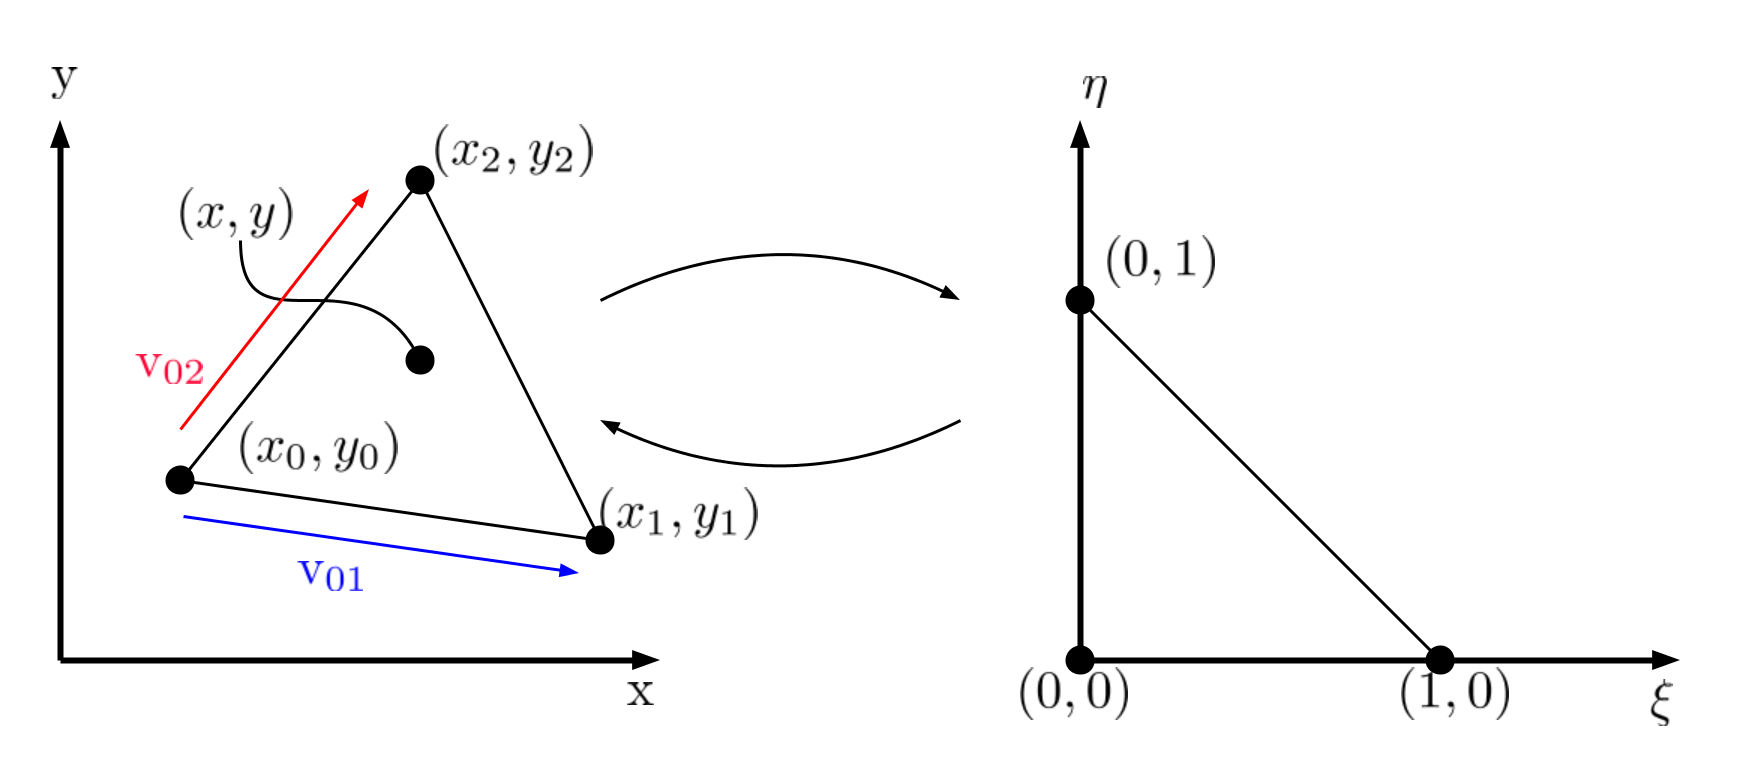
\includegraphics[width=0.7\linewidth]{figures/TwoD_ReferenceElement}
\caption{Triangle reference element.}
\label{fig:twodreferenceelement}
\end{figure}

The linear shape functions on the degrees of freedom of the right reference element are 
\beq 
N_0(\xi,\eta) &= 1 - \xi - \eta \\
N_1(\xi,\eta) &= \xi \\
N_2(\xi,\eta) &= \eta. \\
\eeq 
From these functions we can interpolate the point $(x,y)$ with the following

\beq 
x &= N_0 x_0 + N_1 x_1 + N_2 x_2 \\
y &= N_0 y_0 + N_1 y_1 + N_2 y_2 \\
\eeq 
We can now express $x$ and $y$ as functions of $\xi$ and $\eta$ by substituting the expressions for $N_0$, $N_1$ and $N_2$ into the expressions for $x$ and $y$

\beq 
x &= (1-\xi-\eta)x_0 + (\xi)x_1 + (\eta)x_2 \\
&= x_0 -\xi x_0 -\eta x_0 +\xi x_1 +\eta x_2 \\
&= x_0 +(x_1 - x_0)\xi + (x_2 - x_0)\eta
\eeq 
and
\beq 
y &= (1-\xi-\eta)y_0 + (\xi)y_1 + (\eta)y_2 \\
&= y_0 -\xi y_0 -\eta y_0 +\xi y_1 +\eta y_2 \\
&= y_0 +(y_1 - y_0)\xi + (y_2 - y_0)\eta
\eeq 
\newline
In terms of the vectors from vertex $0$ to the other two vertices (refer to Figure \ref{fig:twodreferenceelement}) we can write this as

\beqn \label{eq:x2Dnat}
x = x_0 + \text{v}_{01x} \xi +\text{v}_{02x} \eta
\eeqn 
\beqn \label{eq:y2Dnat}
y = y_0 + \text{v}_{01y} \xi +\text{v}_{02y} \eta
\eeqn 
\newline
which is in the form of a linear transformation and from which we can determine the very important Jacobian matrix

\begingroup
\renewcommand*{\arraystretch}{1.5}
\beqn \label{eq:jacobiantriangle} 
\mathbf{J }= 
\begin{bmatrix}
\dfrac{dx}{d\xi}     & \dfrac{dx}{d\eta} \\
\dfrac{dy}{d\xi}     & \dfrac{dy}{d\eta} \\
\end{bmatrix}=
\begin{bmatrix}
\text{v}_{01x}  & \text{v}_{02x}  \\
\text{v}_{01y}  & \text{v}_{02y}  \\
\end{bmatrix}
=
\begin{bmatrix}
(x_1 - x_0) & (x_2 - x_0)  \\
(y_1 - y_0)  & (y_2 - y_0) \\
\end{bmatrix}.
\eeqn
\endgroup
\newline
\newline
From which we can determine any transformation

\begin{equation}
\begin{bmatrix}
x \\ y
\end{bmatrix}
=
\vec{\text{v}}_0 + \mathbf{J}
\begin{bmatrix}
\xi \\ \eta
\end{bmatrix}
= \vec{\text{v}}
\end{equation}
and 
\begin{equation}
\begin{bmatrix}
\xi \\ \eta
\end{bmatrix}
= \mathbf{J}^{-1}
\biggr[\vec{\text{v}} -
\vec{\text{v}}_0
\biggr].
\end{equation}

Therefore, given any position in cartesian coordinates (i.e. $xy$), we can use the transformation above to obtain the corresponding natural coordinates $\xi$ and $\eta$ and subsequently evaluate the value of the shape function. Using this approach we can see the shape functions on a triangle in Figure \ref{fig:shapefunctiontri} below.

\begin{figure}[H]
\centering
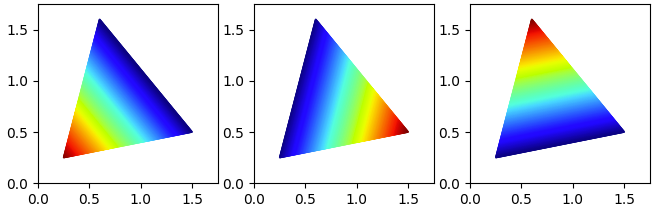
\includegraphics[width=0.7\linewidth]{figures/ShapeFunctionTri.png}
\caption{Linear shape functions on a triangle.}
\label{fig:shapefunctiontri}
\end{figure}


\newpage 
\begin{thebibliography}{1}
    
    \bibitem{OldRMC} Zhang Y., Morel J.E., {\em Transport Error Estimation via Non-Recursive Residual Monte Carlo}, PHYSOR 2018, April 2018
    
    \bibitem{ChiTech} Vermaak J.I.C., {\em $\chi$-Tech: A large-scale scientific simulation engine being developed at Texas A\&M University as part of a research study}, \url{https://github.com/chi-tech/chi-tech}
    
    
\end{thebibliography}

\end{document}